\chapter{Numerical results}
We have implemented the Finite Volume Method for solving the shallow water equations in 1D and tested it on two different dam break problems
\footnote{Code and small animations can be found at github, visit \url{https://github.com/MelissaJessen/Shallow-Water-Equations}.}.

\section{Metod of manufactured solutions}
Method of manufactured solutions (MMS) was used to verify the implementation.
We use a manufactured solution for $h(x,t)$ and $u(x,t)$.
Choose a simple sine wave function for the water height $h$ and a corresponding $u$ that satisfies the shallow water equations.
Consider
\begin{align*}
    h(x,t) &= h_0 + A \cos(\omega t - kx), \\
    u(x,t) &= \frac{ A \omega }{k h_0}  \cos(\omega t - kx),
\end{align*} 
where $h_0$ is the constant base depth, $A$ is the amplitude of the wave, $k$ is the wave number, and $\omega$ is the angular frequency.

We begin by computing the source terms $S_h$ and $S_u$.
First we compute the partial derivatives
\begin{align*}
    h_t &= ,\\
    u_t &=  \\
\end{align*}
which gives (using the chain rule)
\begin{align*}
    {(hu)}_x &= h_x u + h u_x \\
    &= 
\end{align*}

\section{The 1D Dam Break Problem}
The numerical solution to the 1D Dam Break Problem using the FVM, together with the true solution can be seen in \autoref{fig:1D_dam_break}.

\begin{figure}[H]
    \centering
    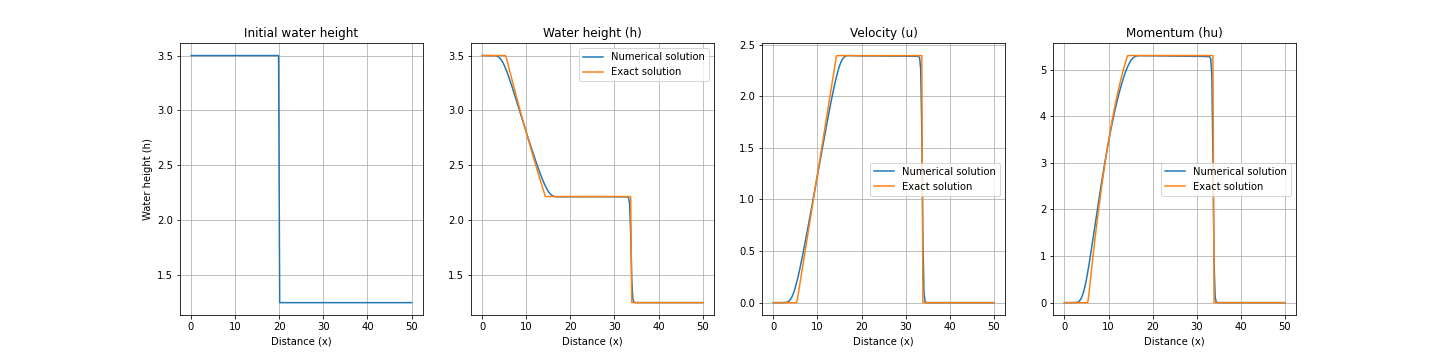
\includegraphics[width=0.8\textwidth]{plots/sol_1D_val.png}
    \caption{1D dam break problem.}\label{fig:1D_dam_break}
\end{figure}


\subsection{Toro test cases}
We have tested the implementation on the five test cases from Toro's book~\cite{Toro2001-Shock}.
The initial conditions for the five test cases are given in \autoref{tab:toro_test_cases}.

\begin{table}[H]
    \centering
    \begin{tabular}{c|c|c|c|c|c|c}
        \hline
        \textbf{Test case} & \textbf{$h_L$} & \textbf{$u_L$} & \textbf{$h_R$} & \textbf{$u_R$} & \textbf{$x_0$} & \textbf{$t_{end}$} \\
        \hline\hline
        1 & 1.0 & 2.5 & 0.1 & 0.0 & 10.0 & 7.0 \\
        2 & 1.0 & -5.0 & 1.0 & 5.0 & 25.0 & 2.5 \\
        3 & 1.0 & 0.0 & 0.0 & 0.0 & 20.0 & 4.0 \\
        4 & 0.0 & 0.0 & 1.0 & 0.0 & 30.0 & 4.0 \\
        5 & 0.1 & -3.0 & 0.1 & 3.0 & 25.0 & 5.0 \\
        \hline
    \end{tabular}
    \caption{Initial conditions for the five test cases.}
    \label{tab:toro_test_cases}
\end{table}



Test case 1:
\begin{figure}[H]
    \centering
    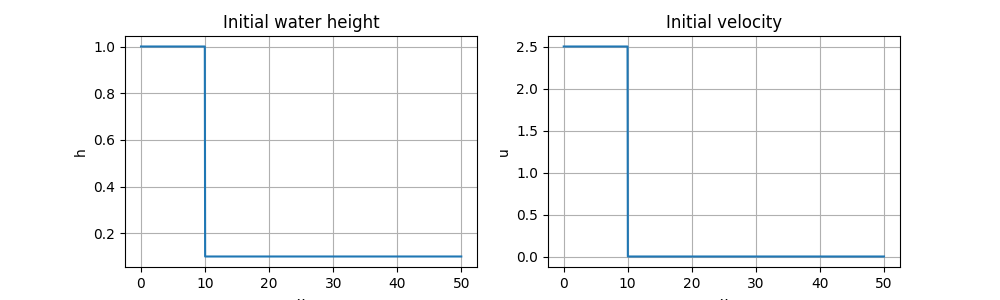
\includegraphics[width=0.7\textwidth]{C:/Users/Matteo/Shallow-Water-Equations/plots/toro_test1_initial.png}
    \caption{Initial conditions for the test case.}\label{fig:toro_test1_initial}
\end{figure}


\begin{figure}[H]
    \centering
    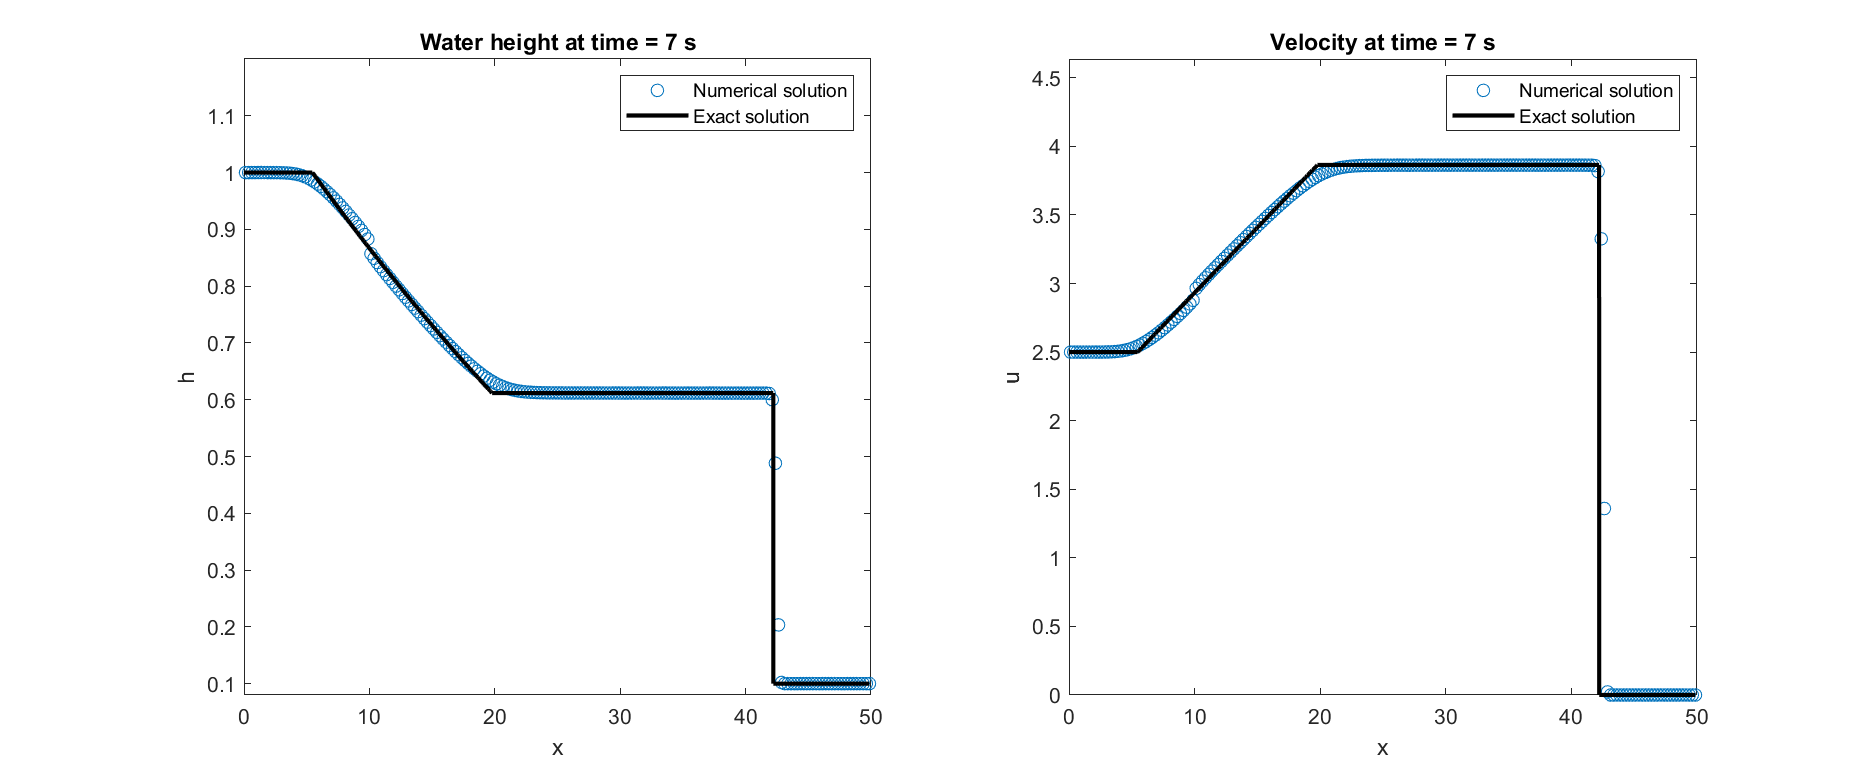
\includegraphics[width=0.7\textwidth]{C:/Users/Matteo/Shallow-Water-Equations/plots/toro_test1_final.png}
    \caption{Final solution for the test case.}\label{fig:toro_test1_final}
\end{figure}


Test case 2: 
\begin{figure}[H]
    \centering
    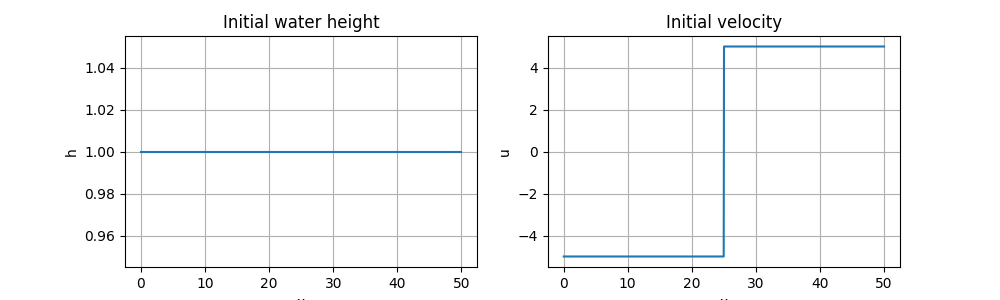
\includegraphics[width=0.7\textwidth]{C:/Users/Matteo/Shallow-Water-Equations/plots/toro_test2_initial.png}
    \caption{Initial conditions for the test case.}\label{fig:toro_test2_initial}
\end{figure}

\begin{figure}[H]
    \centering
    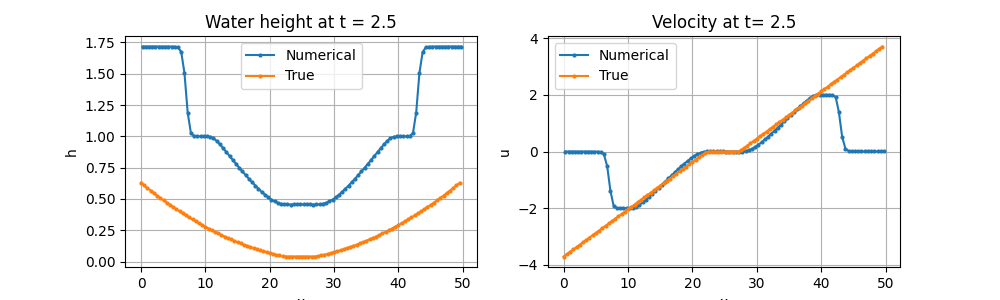
\includegraphics[width=0.7\textwidth]{C:/Users/Matteo/Shallow-Water-Equations/plots/toro_test2_final.png}
    \caption{Final solution for the test case.}\label{fig:toro_test2_final}
\end{figure}


Test case 3:
\begin{figure}[H]
    \centering
    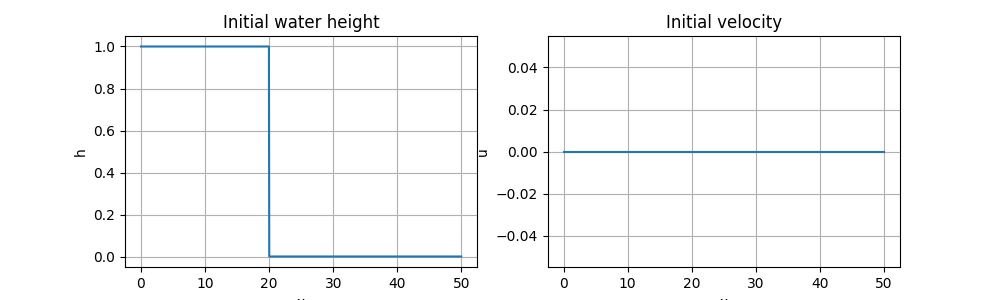
\includegraphics[width=0.7\textwidth]{C:/Users/Matteo/Shallow-Water-Equations/plots/toro_test3_initial.png}
    \caption{Initial conditions for the test case.}\label{fig:toro_test3_initial}
\end{figure}

\begin{figure}[H]
    \centering
    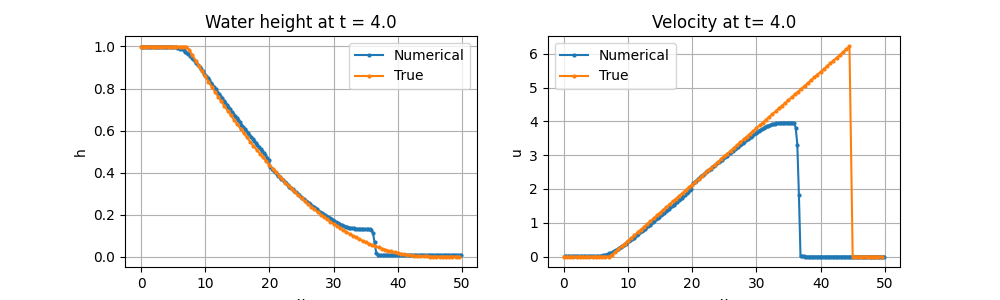
\includegraphics[width=0.7\textwidth]{C:/Users/Matteo/Shallow-Water-Equations/plots/toro_test3_final.png}
    \caption{Final solution for the test case.}\label{fig:toro_test3_final}
\end{figure}
To solve case 3, with the FVM we must add a small amount to $h_R$, since the code does not handle $h_R = 0$ well.
We set $h_R = 0.00005$.
The true solution is for $h_R = 0$.
By running experiments with different values of $h_R$, we see that the solution converges to the true solution as $h_R$ approaches 0.


Test case 4:
\begin{figure}[H]
    \centering
    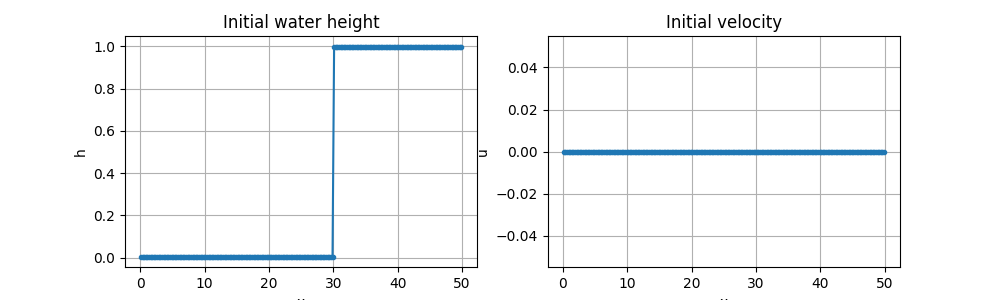
\includegraphics[width=0.7\textwidth]{C:/Users/Matteo/Shallow-Water-Equations/plots/toro_test4_initial.png}
    \caption{Initial conditions for the test case.}\label{fig:toro_test4_initial}
\end{figure}

\begin{figure}[H]
    \centering
    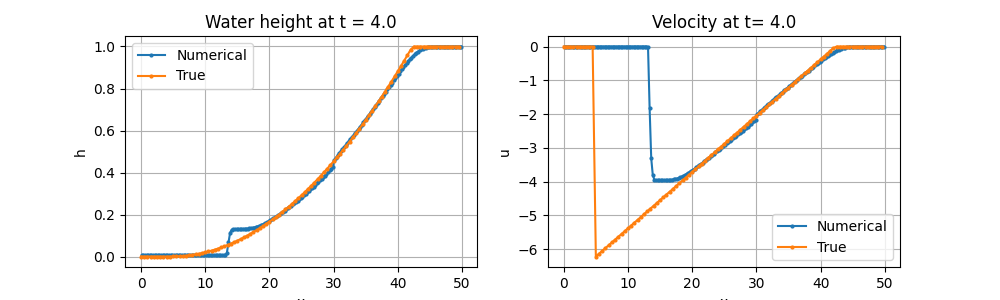
\includegraphics[width=0.7\textwidth]{C:/Users/Matteo/Shallow-Water-Equations/plots/toro_test4_final.png}
    \caption{Final solution for the test case.}\label{fig:toro_test4_final}
\end{figure}
In case 4 we face the same challenges as in case 3.
We set $h_L = 0.00005$, and the solution converges to the true solution as $h_L$ approaches 0.



Test case 5:
\begin{figure}[H]
    \centering
    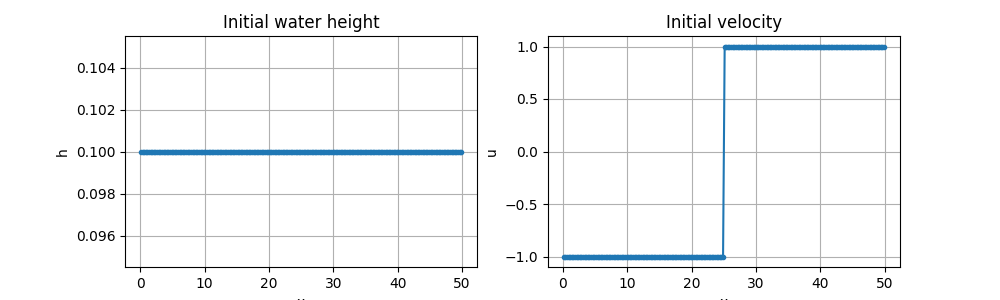
\includegraphics[width=0.7\textwidth]{C:/Users/Matteo/Shallow-Water-Equations/plots/toro_test5_initial.png}
    \caption{Initial conditions for the test case.}\label{fig:toro_test5_initial}
\end{figure}

\begin{figure}[H]
    \centering
    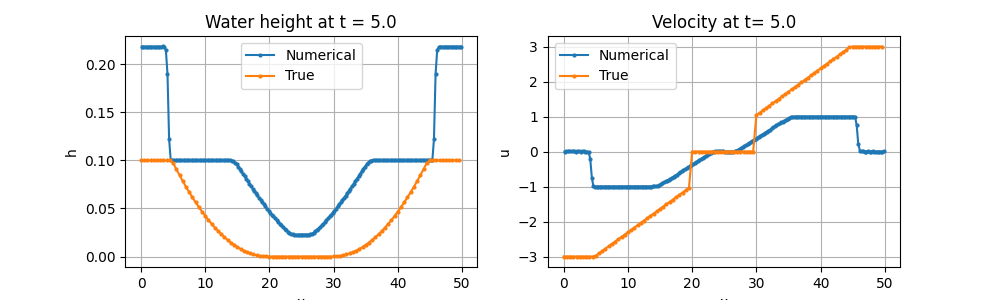
\includegraphics[width=0.7\textwidth]{C:/Users/Matteo/Shallow-Water-Equations/plots/toro_test5_final.png}
    \caption{Final solution for the test case.}\label{fig:toro_test5_final}
\end{figure}
From~\autoref{fig:toro_test5_final} we see that the numerical solutions for the velocity $v$ at $t=5.0$ are smooth, where the true solution is discontinuous. 


\section{2D idealised Circular Dam Break Problem}
Consider the idealised circular dam break problem with a horizontal bottom.
We assume there is an infinitely thin circular wall at radius $R = 2.5 m$ is a square domain of size $40 m \times 40 m$ with centre at $(x_c,y_c) = (20 m, 20 m)$.
The initial conditions are (ch. 15 Toro)
\begin{align*}
    h(x,y,0) &= \begin{cases}
        2.5 \text{ }m, & \text{if } \sqrt{ {(x-x_c)}^2 + {(y-y_c)}^2 } \leq R, \\
        0.5 \text{ }m, & \text{otherwise},
    \end{cases} \\
    u(x,y,0) &= 0, \\
    v(x,y,0) &= 0.
\end{align*}
Use the WAF method (chapter 11) along with a second-order dimensional splitting scheme (chapter 12).
CFL-condition: $C_{cfl} = 0.9$.
van Leer limiter. Mesh: $200 \times 200$.

\begin{figure}[H]
    \centering
    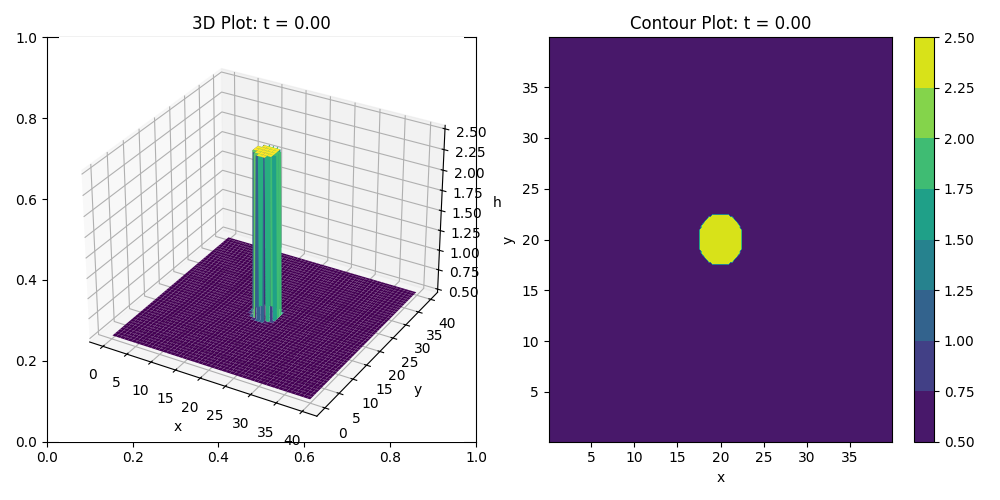
\includegraphics[width=0.6\textwidth]{C:/Users/Matteo/Shallow-Water-Equations/plots/toro2D_t=0.png}
    \caption{2D dam break problem after $t=0$.}\label{fig:2D_dam_break_t0}
\end{figure}

\begin{figure}[H]
    \centering
    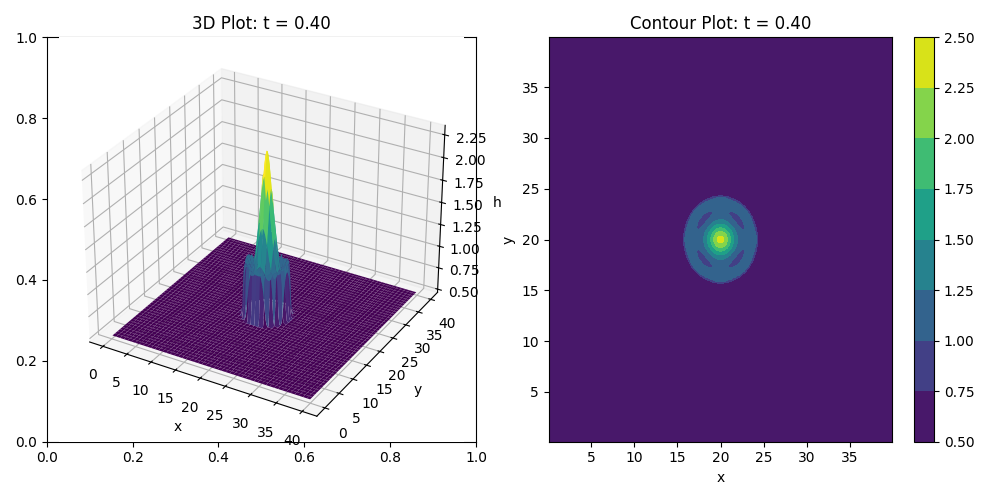
\includegraphics[width=0.6\textwidth]{C:/Users/Matteo/Shallow-Water-Equations/plots/toro2D_t=0.4.png}
    \caption{2D dam break problem after $t=0.4$.}\label{fig:2D_dam_break_t0.4}
\end{figure}

\begin{figure}[H]
    \centering
    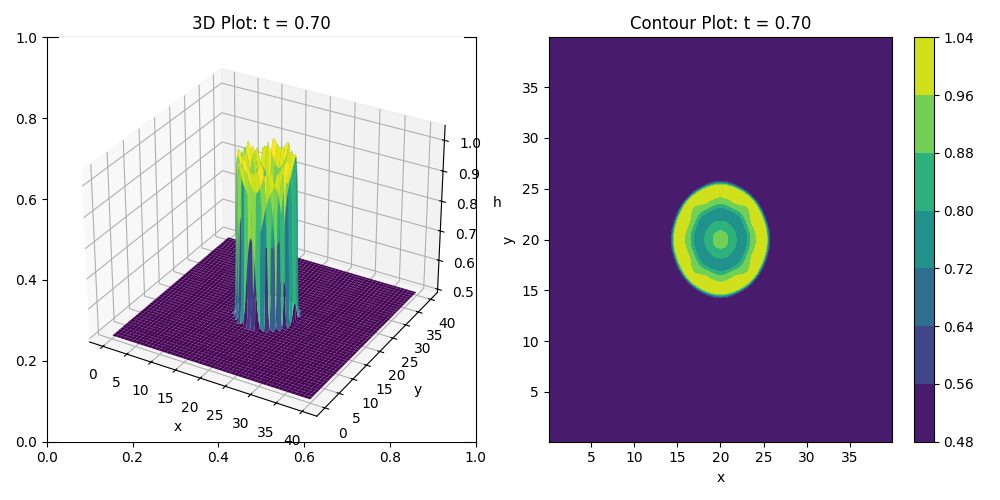
\includegraphics[width=0.6\textwidth]{C:/Users/Matteo/Shallow-Water-Equations/plots/toro2D_t=0.7.png}
    \caption{2D dam break problem after $t=0.7$.}\label{fig:2D_dam_break_t0.7}
\end{figure}

\begin{figure}[H]
    \centering
    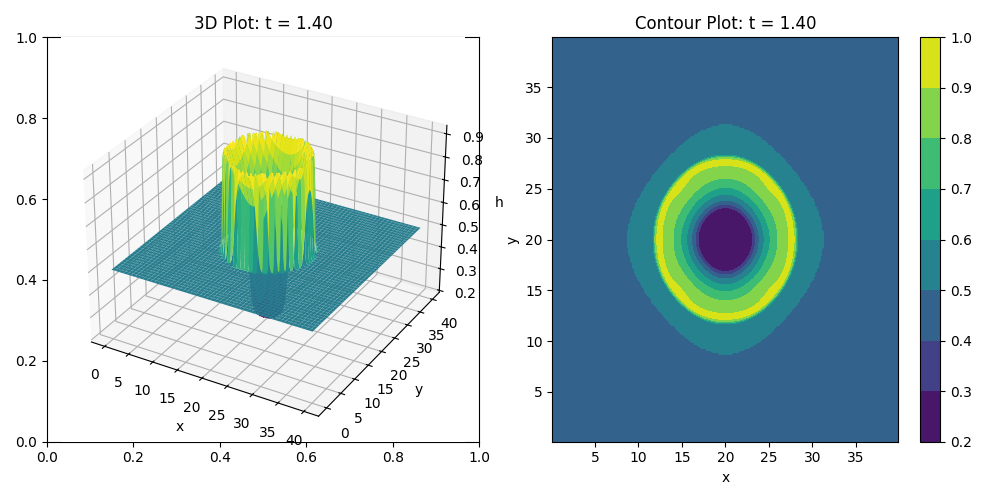
\includegraphics[width=0.6\textwidth]{C:/Users/Matteo/Shallow-Water-Equations/plots/toro2D_t=1.4.png}
    \caption{2D dam break problem after $t=1.4$.}\label{fig:2D_dam_break_t1.4}
\end{figure}




